\section{Dados}

\subsection{Dados originais}
Os dados usados neste estudo foram obtidos e proporcionados pela \textit{Evoluation AI} \footnote{Os dados podem ser encontrados em: \url{https://www.kaggle.com/mswarbrickjones/reddit-selfposts}}. Estes consistem em \textit{self-posts} feitos no \textit{Reddit} entre 2016/06/01 e 2018/06/01 (2 anos). De forma a garantir alguma qualidade, os dados foram submetidos a filtragem por parte da \textit{Evoluation AI}:
\begin{itemize}
    \item \textit{Posts} submetidas noutra língua que não o inglês.
    \item \textit{Posts} submetidos por moderadores ou \textit{admins} do \textit{Reddit}.
    \item \textit{Posts} cujo corpo de texto possuísse menos do que 256 ou mais do que 4096 caracteres.
    \item \textit{Posts} duplicados.
\end{itemize}

Desta maneira, o \textit{dataset} final é constituído por postagens de 1013 classes, sendo que cada uma possui 1000 postagens. Mais informações sobre o tratamento ao qual os dados foram submetidos ou sobre algum estudo feito sobre eles podem ser encontradas em \cite{data_paper}. As classes são, por isso, o nome dos \textit{subreddits} i.e., um dado tema, e cada uma possui 1000 postagens (exemplos) feitas nesse \textit{subreddit}.

\subsection{Divisão dos dados para o estudo}
\label{subsub:data_initial_division}

Apesar do \textit{dataset} original possuir 1013 classes distintas, por uma questão de \textit{hardware constraints}, decidimos usar apenas 50 para realizar o nosso estudo, sendo que a selecção das mesmas foi feita de forma aleatória. Desta forma, todo o trabalho foi feito usando 50 mil exemplos de \textit{posts} distintos, já que cada classe, como já referido, possui 1000 amostras. 

Como recomendação dos proprietários do \textit{dataset}, usamos a divisão 80\%-20\% para dados de treino/\textit{cross validation} e de teste, já que os dados originais se encontravam organizados de forma a que, com esta divisão, houvessem exactamente 800 amostras para treino/\textit{cross validation} e 200 amostras para teste em cada classe distinta. Nos gráficos da figura \ref{fig:data_distribution} é possível verificar a uniformidade esta distribuição.


\begin{figure*}[!t]
	\centering
	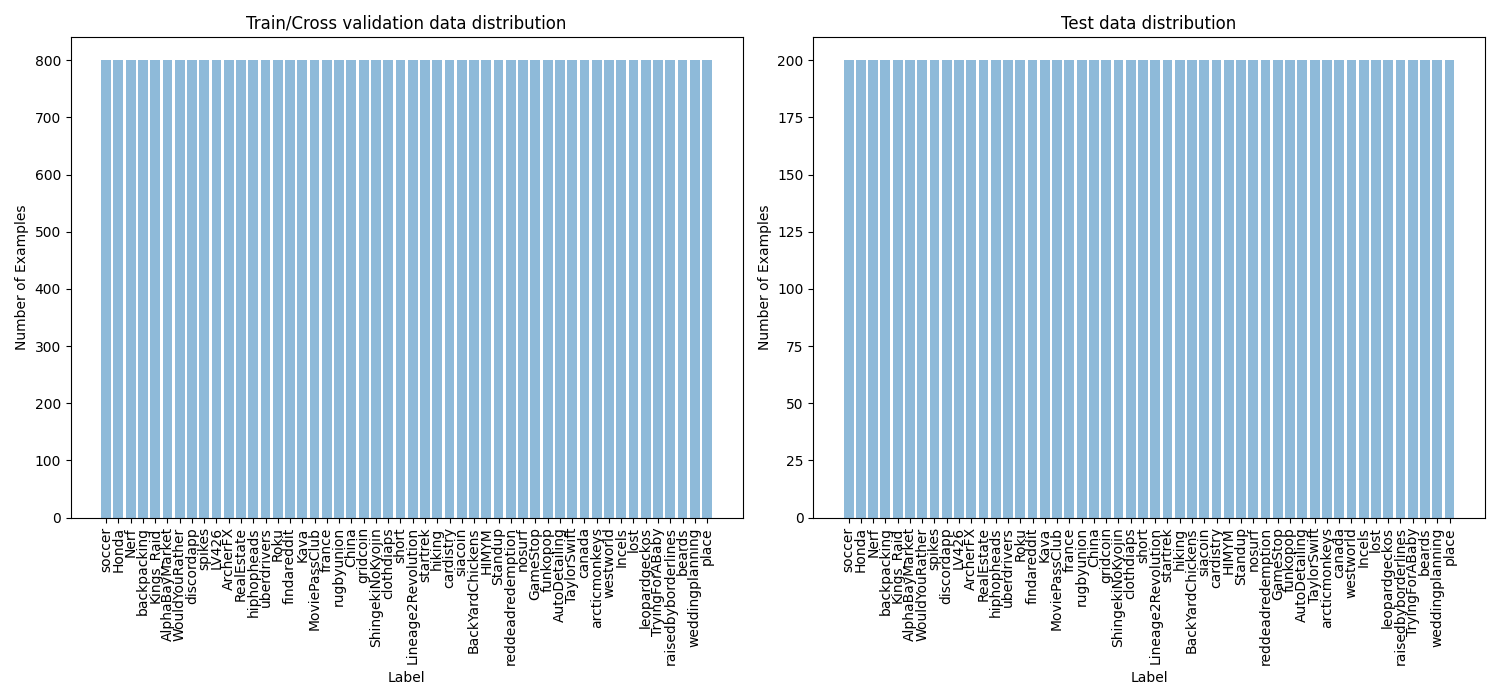
\includegraphics[width=\textwidth]{all_distribution}
	\caption{Distribuição de dados por \textit{label} (nomes dos \textit{subreddits}) por \textit{dataset}.}
	\label{fig:data_distribution}
\end{figure*}


\subsection{Pré-processamento dos dados}
\label{subsub:data_pre_processing}

Sabendo que este trabalho se trata de um problema de \textbf{classificação de texto}, é inevitável que exista algum processamento dos dados de entrada (textos), já que a maioria dos modelos existentes não são compatíveis com entradas não numéricas. Para além de questões de conveniência, nesta etapa também é implementado um mecanismo de escolha de \textit{features}.

Para uma fácil compreensão dos mecanismos usados neste passo, a explicação vai ser feita de uma forma enumerada:
\begin{enumerate}
\item \textbf{Conversão de texto para \textit{tokens}}: Nesta fase os textos presentes no \textit{dataset} são transformados numa lista de \textit{tokens}:
\begin{itemize}
\item Divisão do texto numa lista de \textit{tokens}. Ex.: word\textunderscore{tokenize}("At eight o'clock on Thursday morning.") = ['At', 'eight', "o'clock", 'on', 'Thursday', 'morning', '.'].
\item Todos os \textit{tokens} são convertidos para letra minúscula.
\item Pontuação é removida.
\item É realizado o processo de lematização nos verbos presentes. Ex: inflected: inflect, ate: eat.
\item São retirados os \textit{tokens} que estão incluídos no conjunto de \textit{stop words} inglesas.

\bigbreak
Supondo o seguinte cenário, em que se pretende converter o texto \textit{"Lemmatisation (or lemmatization) in linguistics is the process of grouping together the inflected forms of a word"} para uma lista de \textit{tokens} o \textit{output} esperado seria: ['lemmatisation', 'lemmatization', 'linguistics', 'process', 'group', 'together', 'inflect', 'form', 'word']
\end{itemize}

\bigbreak
\item \textbf{Conversão da lista de \textit{tokens} para uma matriz de \textit{TF-IDF features}}.
Apesar da transformação anterior em \textit{tokens}, é necessário uma nova etapa para conseguir extrair \textit{features} dos textos disponibilizados, para que estes sejam usados à posteriori nos modelos de \textit{Machine Learning} em estudo. Para isso foi usado o algoritmo \textit{\textbf{TF*IDF}}, que é uma técnica de extracção de informação que pesa a frequência de um termo (\textbf{\textit{TF}}) i.e, o número de vezes que o termo aparece, e a frequência inversa de documento (\textbf{\textit{IDF}}) i.e, uma pontuação que define o quão importante é um termo relativamente ao \textit{corpus} total. O produto das pontuações \textbf{\textit{TF}} e \textbf{\textit{IDF}} de um termo é chamado de peso \textbf{\textit{TF*IDF}}. A importância do termo no \textit{corpus} cresce com o aumento da pontuação \textbf{\textit{TF*IDF}} do respectivo termo.

Para mais detalhes, é favor consultar \cite{TF_IDF_algorithm}.

Apenas de referir que nesta etapa foram considerados todos os uni-gramas e bigramas \footnote{\textbf{n-grama}: É uma sequência contínua de \textbf{N} itens de uma determinada amostra de texto. Neste caso foram considerados n = 1 e n = 2}. Após o processo estar completo este algoritmo retorna um conjunto de termos (palavras) com o respectivo valor \textbf{\textit{TF*IDF}} mapeado. Este conjunto de palavras define o vocabulário do nosso \textit{corpus}. 

\bigbreak
\item \textbf{Diminuição do vocabulário proveniente do algoritmo \textit{TF*IDF}}: O conjunto de palavras definido anteriormente reflecte a quantidade de \textit{features} de entrada para o nosso modelo, sendo que, como é expectável, este pode possuir dimensões elevadas. Devido a este facto, é essencial reduzir o numero de \textit{features} (numero de termos do vocabulário), para que os processos de treino sejam optimizados e para cumprir limitações de \textit{hardware}. Apesar de aparentar que podemos retirar informação importante do nosso \textit{corpus}, a diminuição do vocabulário torna-se pouco influente se removermos os termos com valor baixo de \textbf{\textit{TF*IDF}} (termos que não transmitem informação útil sobre o \textit{corpus}). 

Ordenando os termos de vocabulário por ordem decrescente do valor de \textbf{\textit{TF*IDF}}, obtemos um gráfico como o apresentado na figura \ref{diagram:data_n_knee}. Como se pode observar, este possui uma forma exponencial, sendo que os valores mais à esquerda (com maior valor de \textbf{\textit{TF*IDF}}) representam as palavras mais importantes no \textit{corpus} que são, por isso, as palavras mais importantes. Aqui reforça-se a ideia da necessidade de segmentar o vocabulário, pois este atinge dimensões na ordem dos milhões.

\begin{figure}[t]
\begin{center}
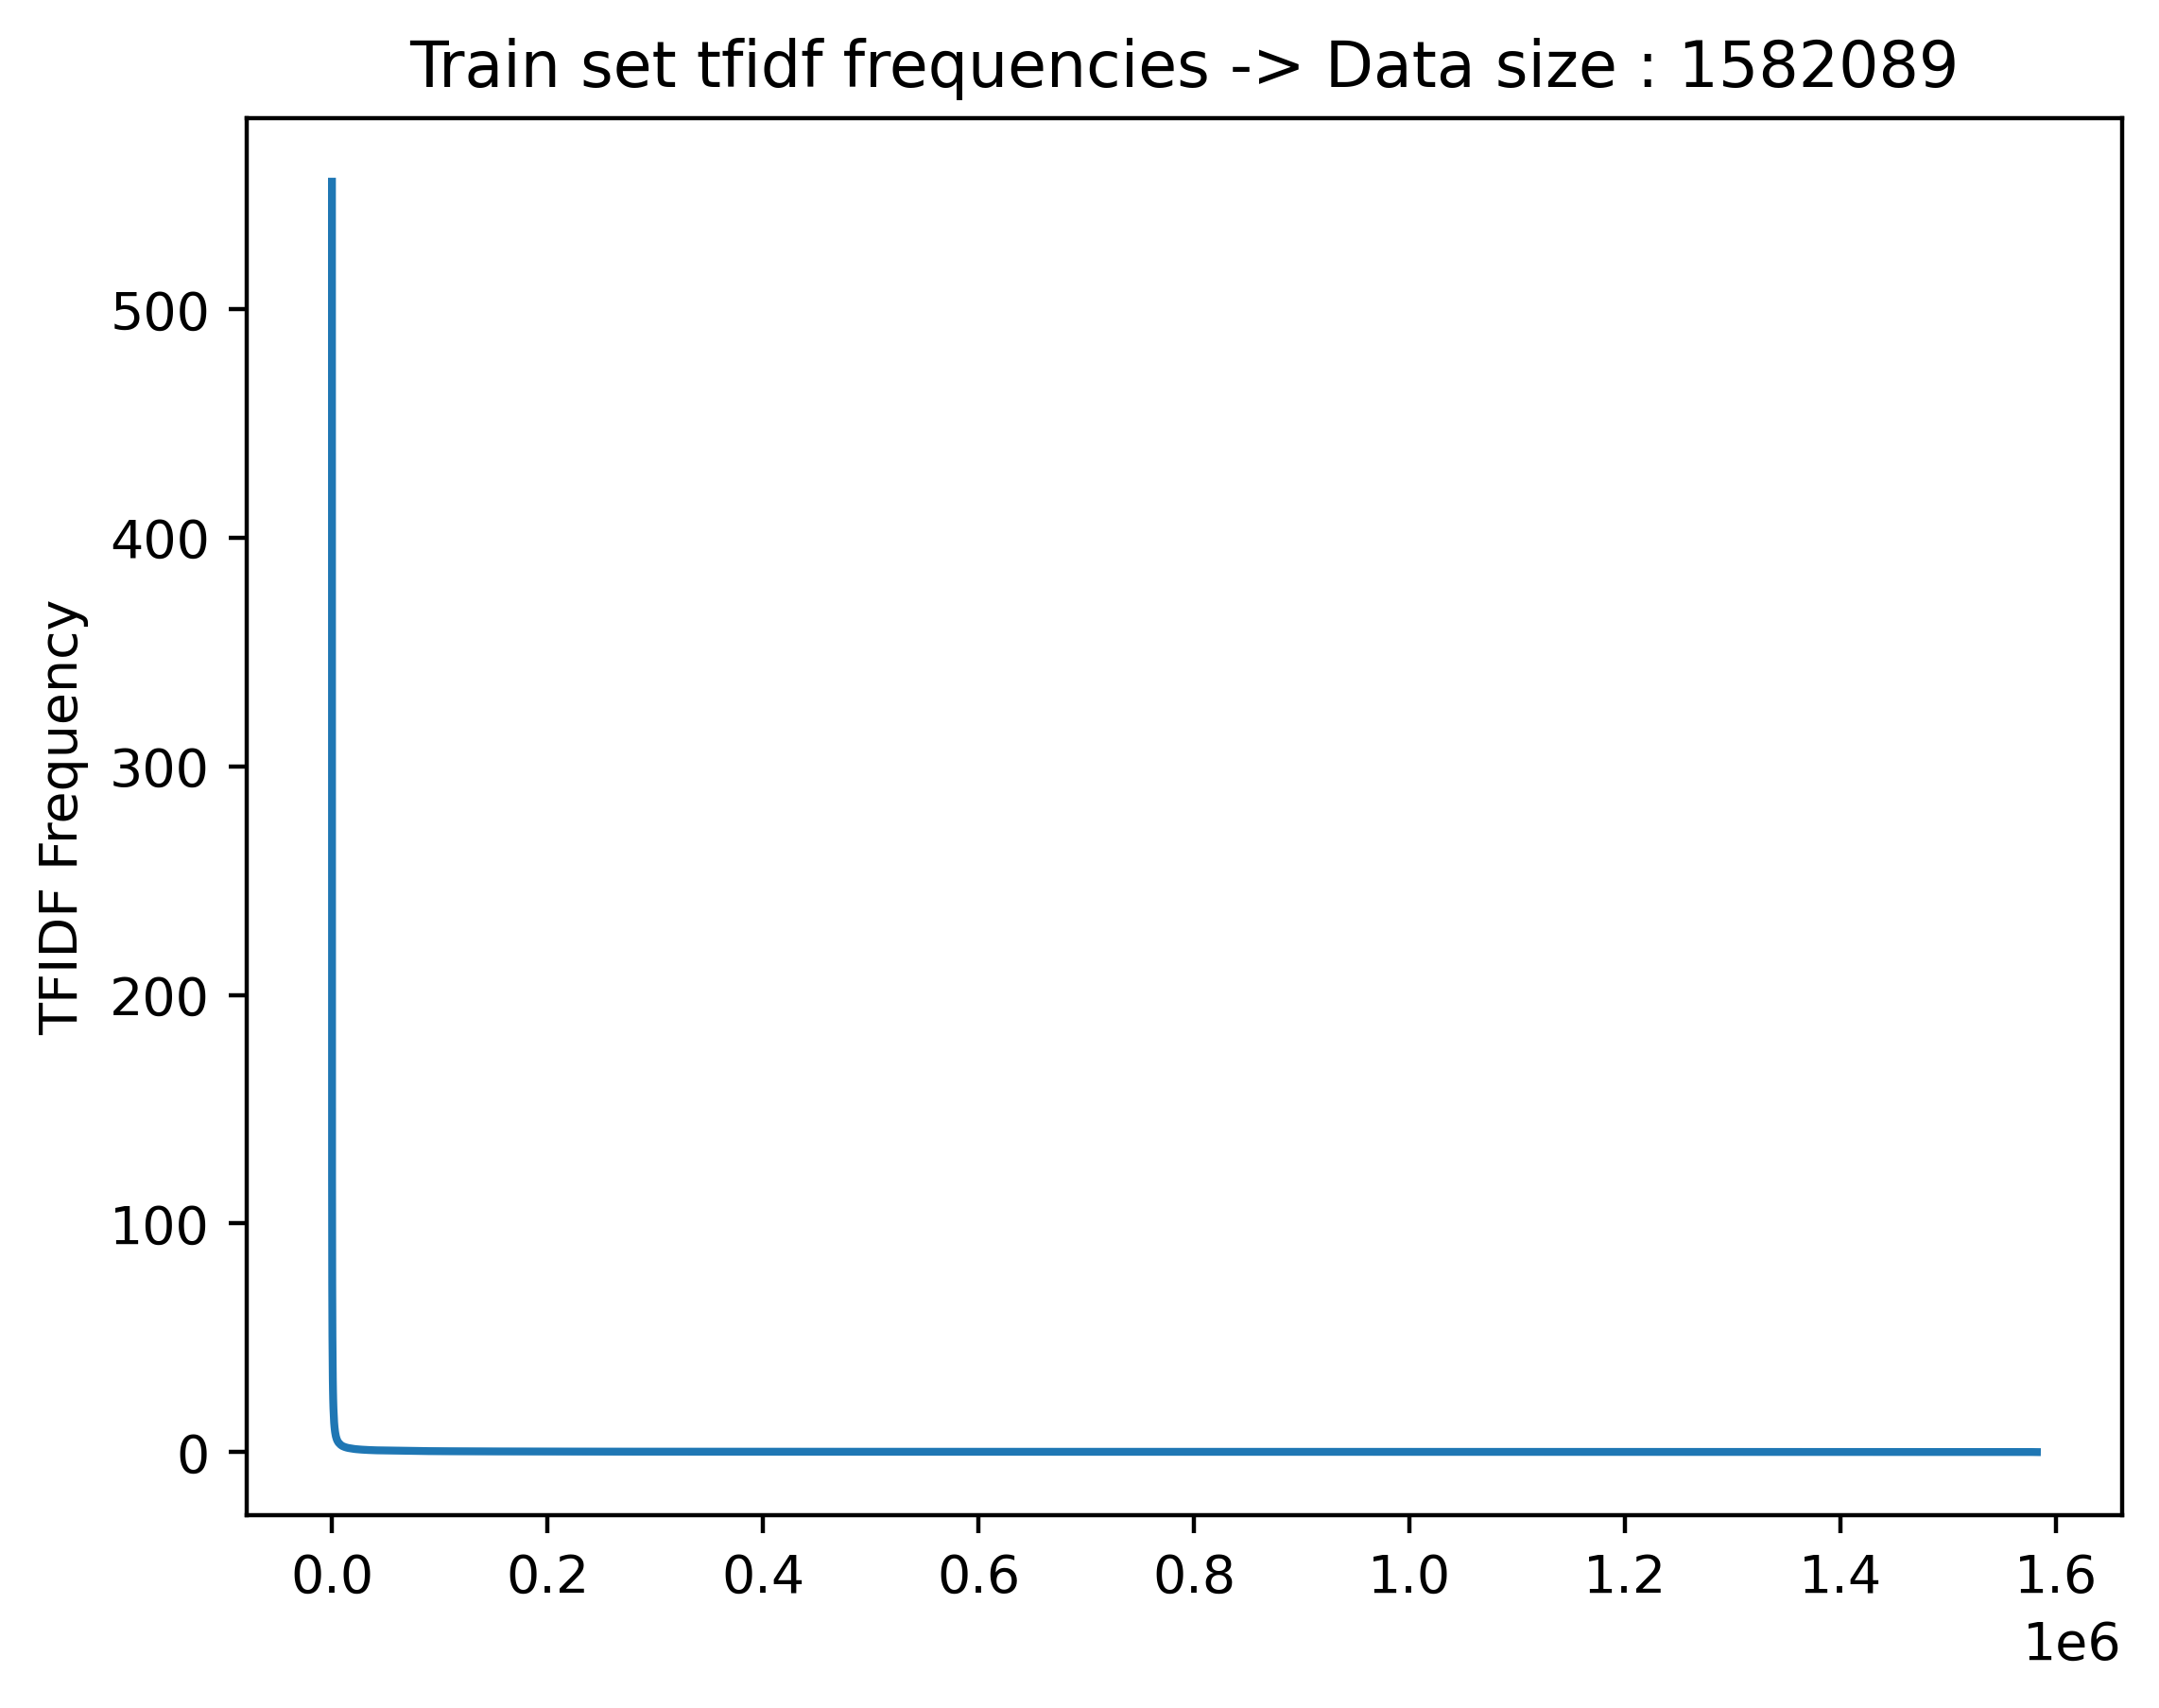
\includegraphics[width=0.5\textwidth,keepaspectratio]{figures/data_n_knee.png}
\caption{Frequências TF*IDF do corpus ordenados de forma decrescente }
\label{diagram:data_n_knee}
\centering
\end{center}
\end{figure}

Para conseguirmos segmentar os termos do vocabulário, tendo em conta a forma de exponencial que este apresenta, foi usado o algoritmo \textit{Kneedle} \cite{Kneedle}, que tem como objectivo seleccionar o ponto onde o vocabulário "deve ser cortado", sendo o ponto ideal o "joelho" (\textit{knee}) do gráfico. Basicamente o algoritmo escolhe o ponto ideal que divide os termos importantes dos não importantes.

Na figura \ref{diagram:data_knee}, podemos observar o \textit{knee\textunderscore{point}} que o algoritmo seleccionou, 7299. Isto implica uma redução de 99\% no tamanho do vocabulário inicial. 

\begin{figure}[t]
\begin{center}
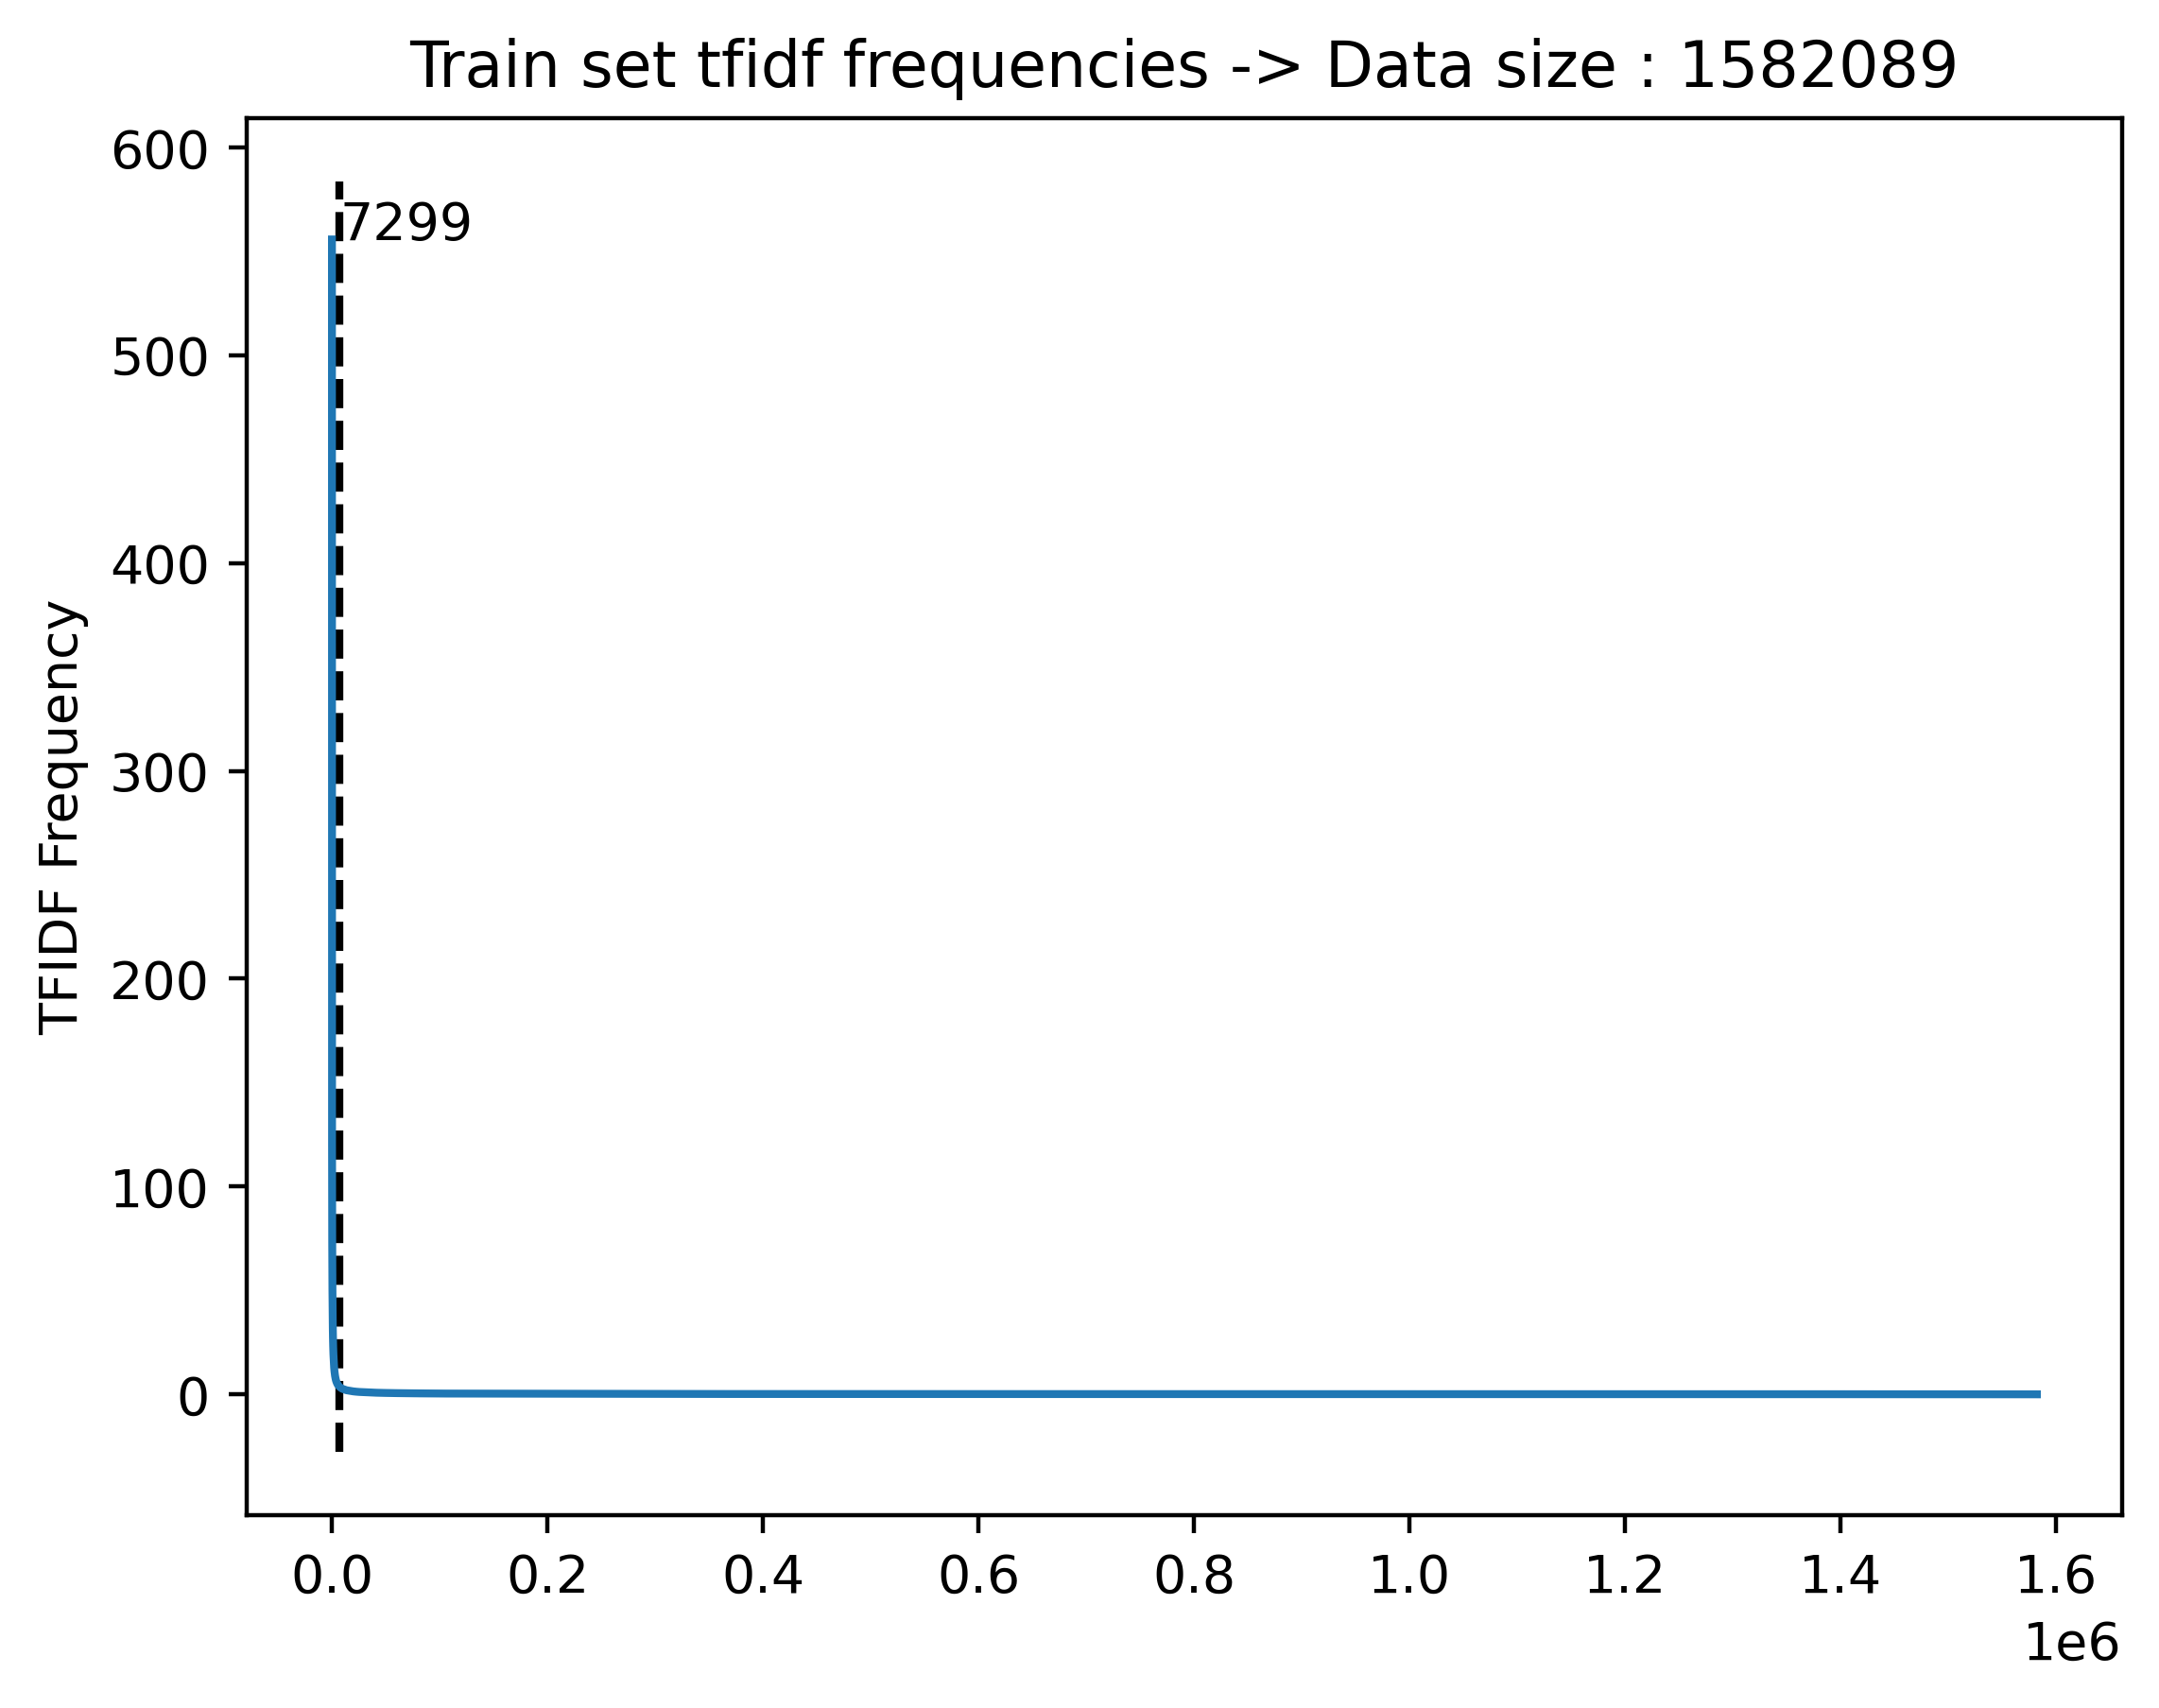
\includegraphics[width=0.5\textwidth,keepaspectratio]{figures/data_knee.png}
\caption{Frequências TF*IDF do corpus ordenados de forma decrescente com o \textit{knee\textunderscore{point}}}
\label{diagram:data_knee}
\centering
\end{center}
\end{figure}

Apesar da redução ser bastante significativa, 7299 termos de vocabulário continua a ser um número elevado de \textit{features}, sendo que para isso uma nova segmentação é realizada com o novo vocabulário reduzido. Como demonstrado na figura \ref{diagram:data_second_knee},  o novo vocabulário continua com a forma de exponencial. Posto isto, este processo é realizado até o algoritmo não conseguir encontrar o \textit{knee point} - este processo pode ser visualizado no gráfico \ref{diagram:data_all_knee}.

\begin{figure}[t]
\begin{center}
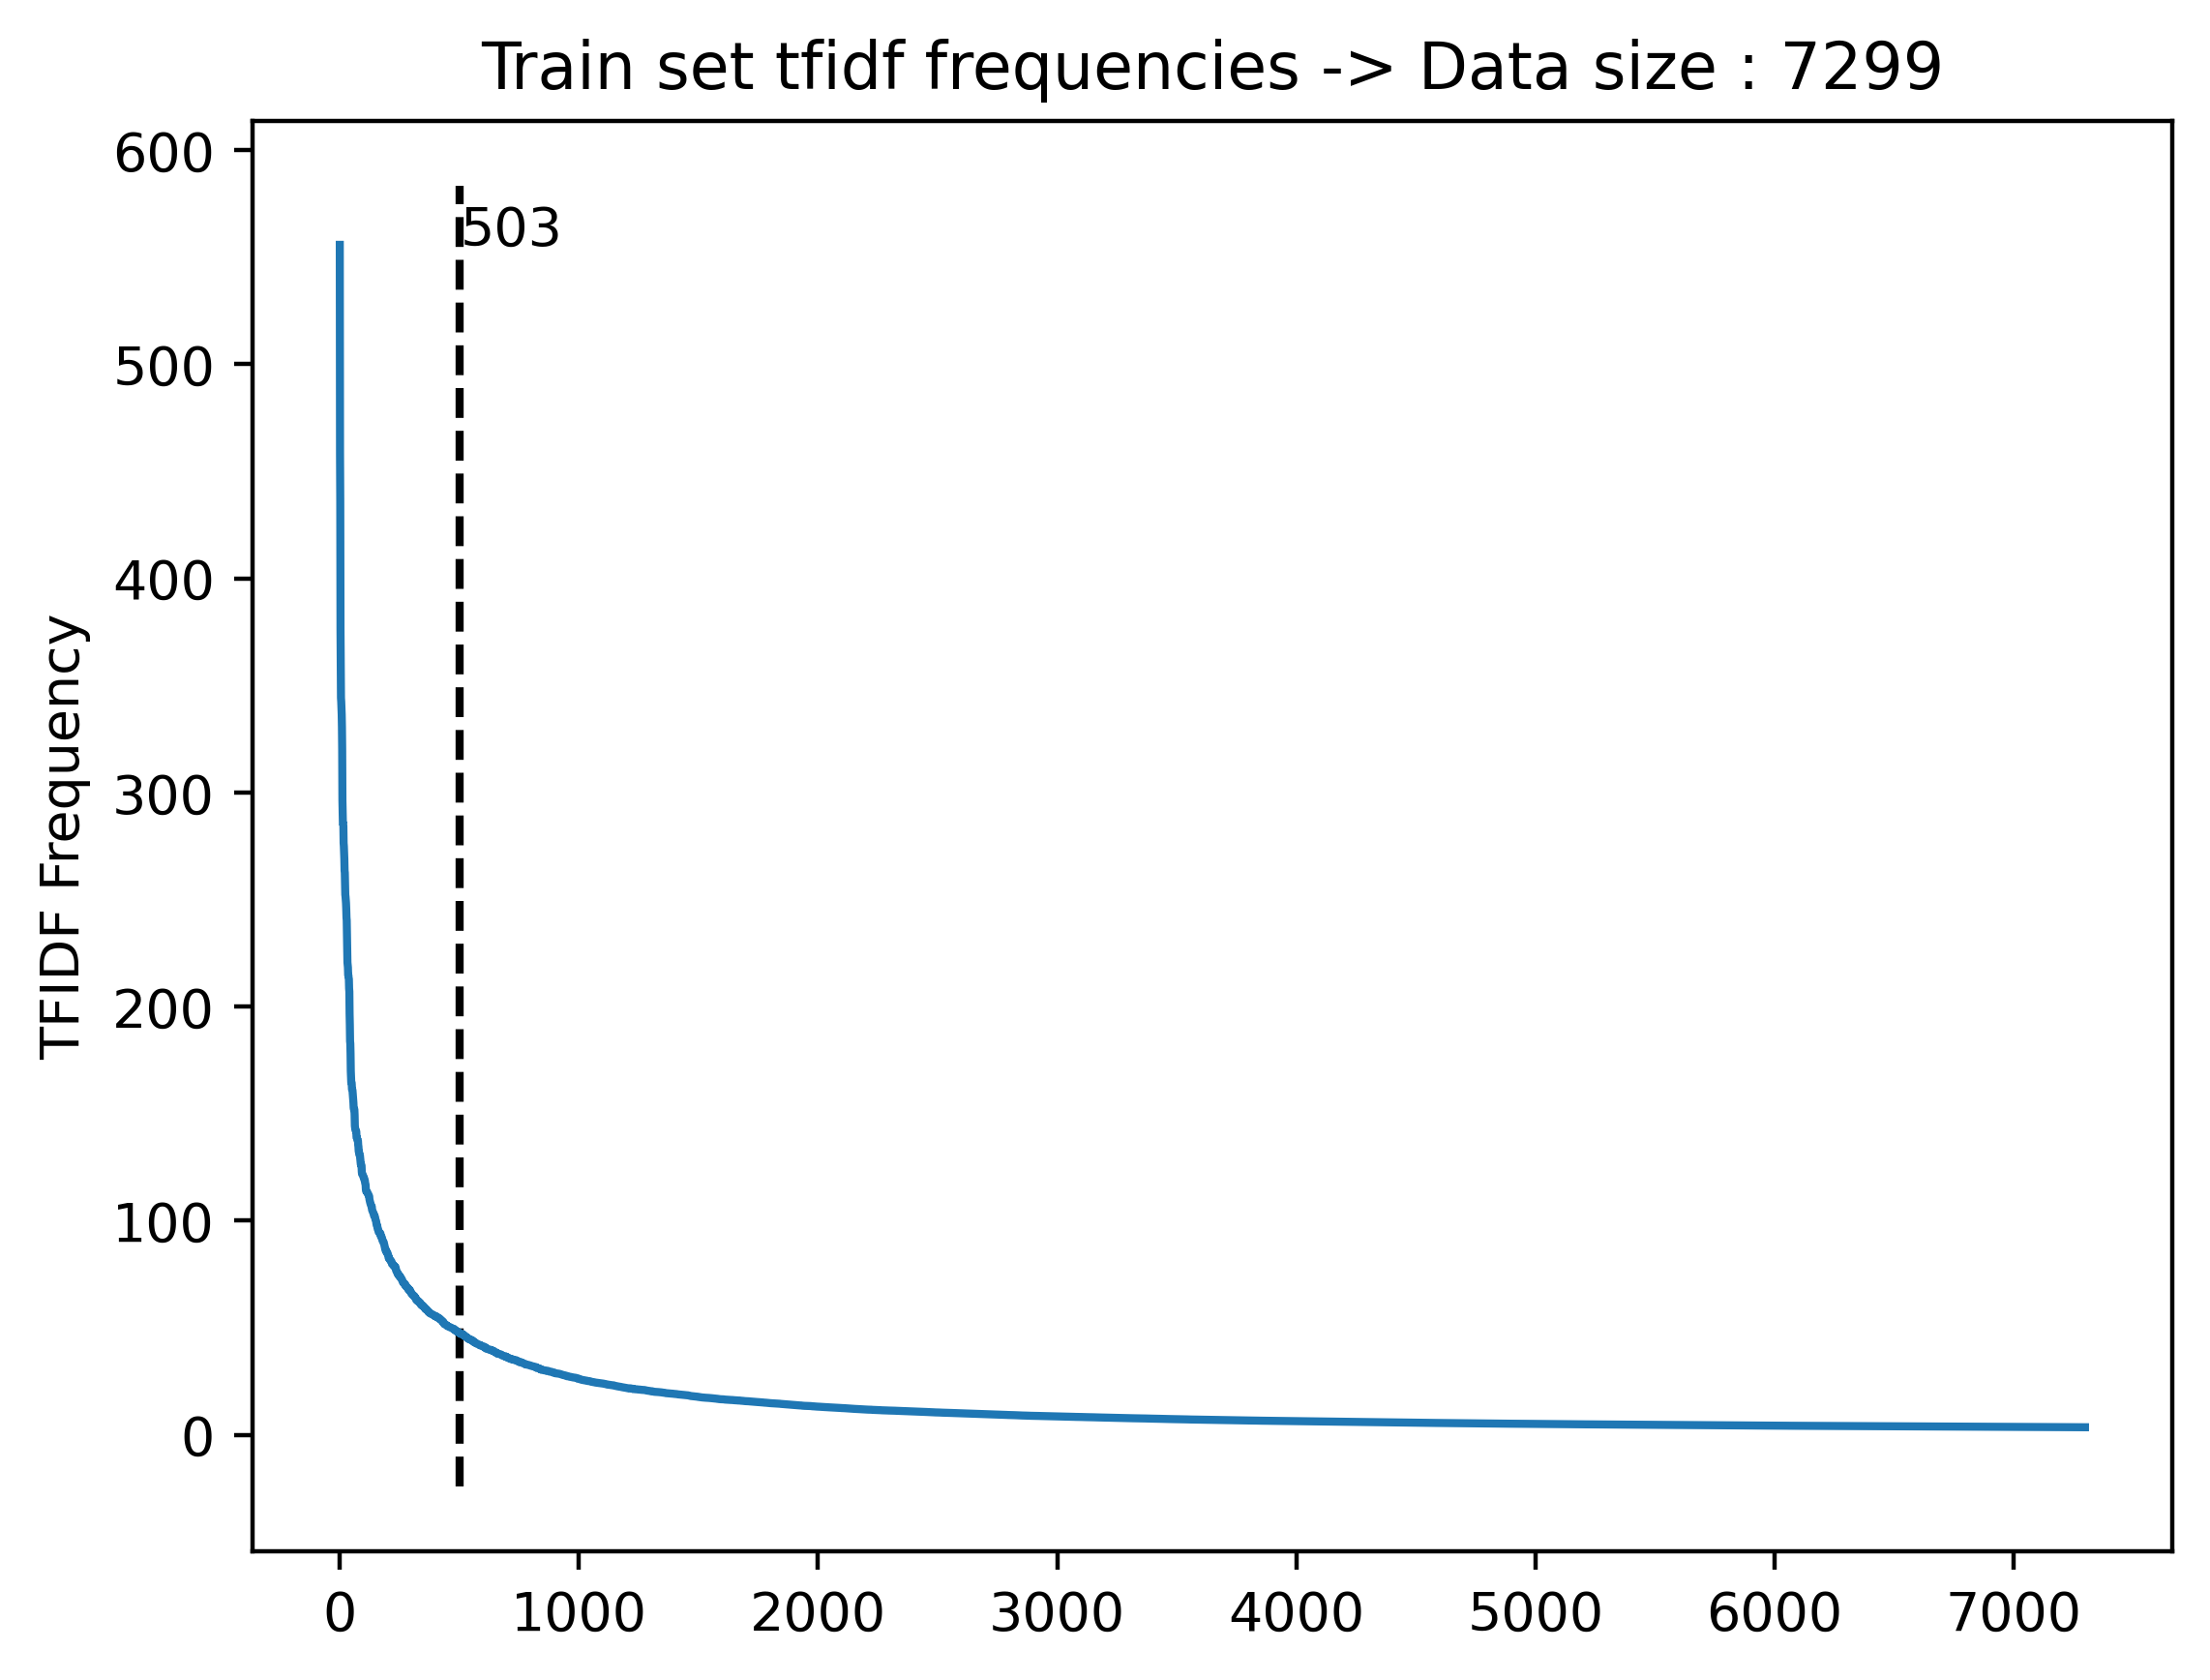
\includegraphics[width=0.5\textwidth,keepaspectratio]{figures/data_size_503.png}
\caption{Frequências TF*IDF do corpus reduzido ordenados de forma decrescente com o \textit{knee\textunderscore{point}}}
\label{diagram:data_second_knee}
\centering
\end{center}
\end{figure}

Como se pode observar, caso a segmentação de dados chegue ao fim, na ultima iteração deste procedimento, o numero de \textit{features} é muito reduzido (11), o que não permite ao modelo obter informação suficiente sobre os documentos. Para evitar isto, foi implementado um parâmetro de limite, que define o numero mínimo de termos que o vocabulário deve ter. Por exemplo, se o limite for de 90 termos, o processo terminaria no terceiro gráfico da figura \ref{diagram:data_all_knee} e o vocabulário ficaria com 93 termos.

\begin{figure}[t]
\begin{center}
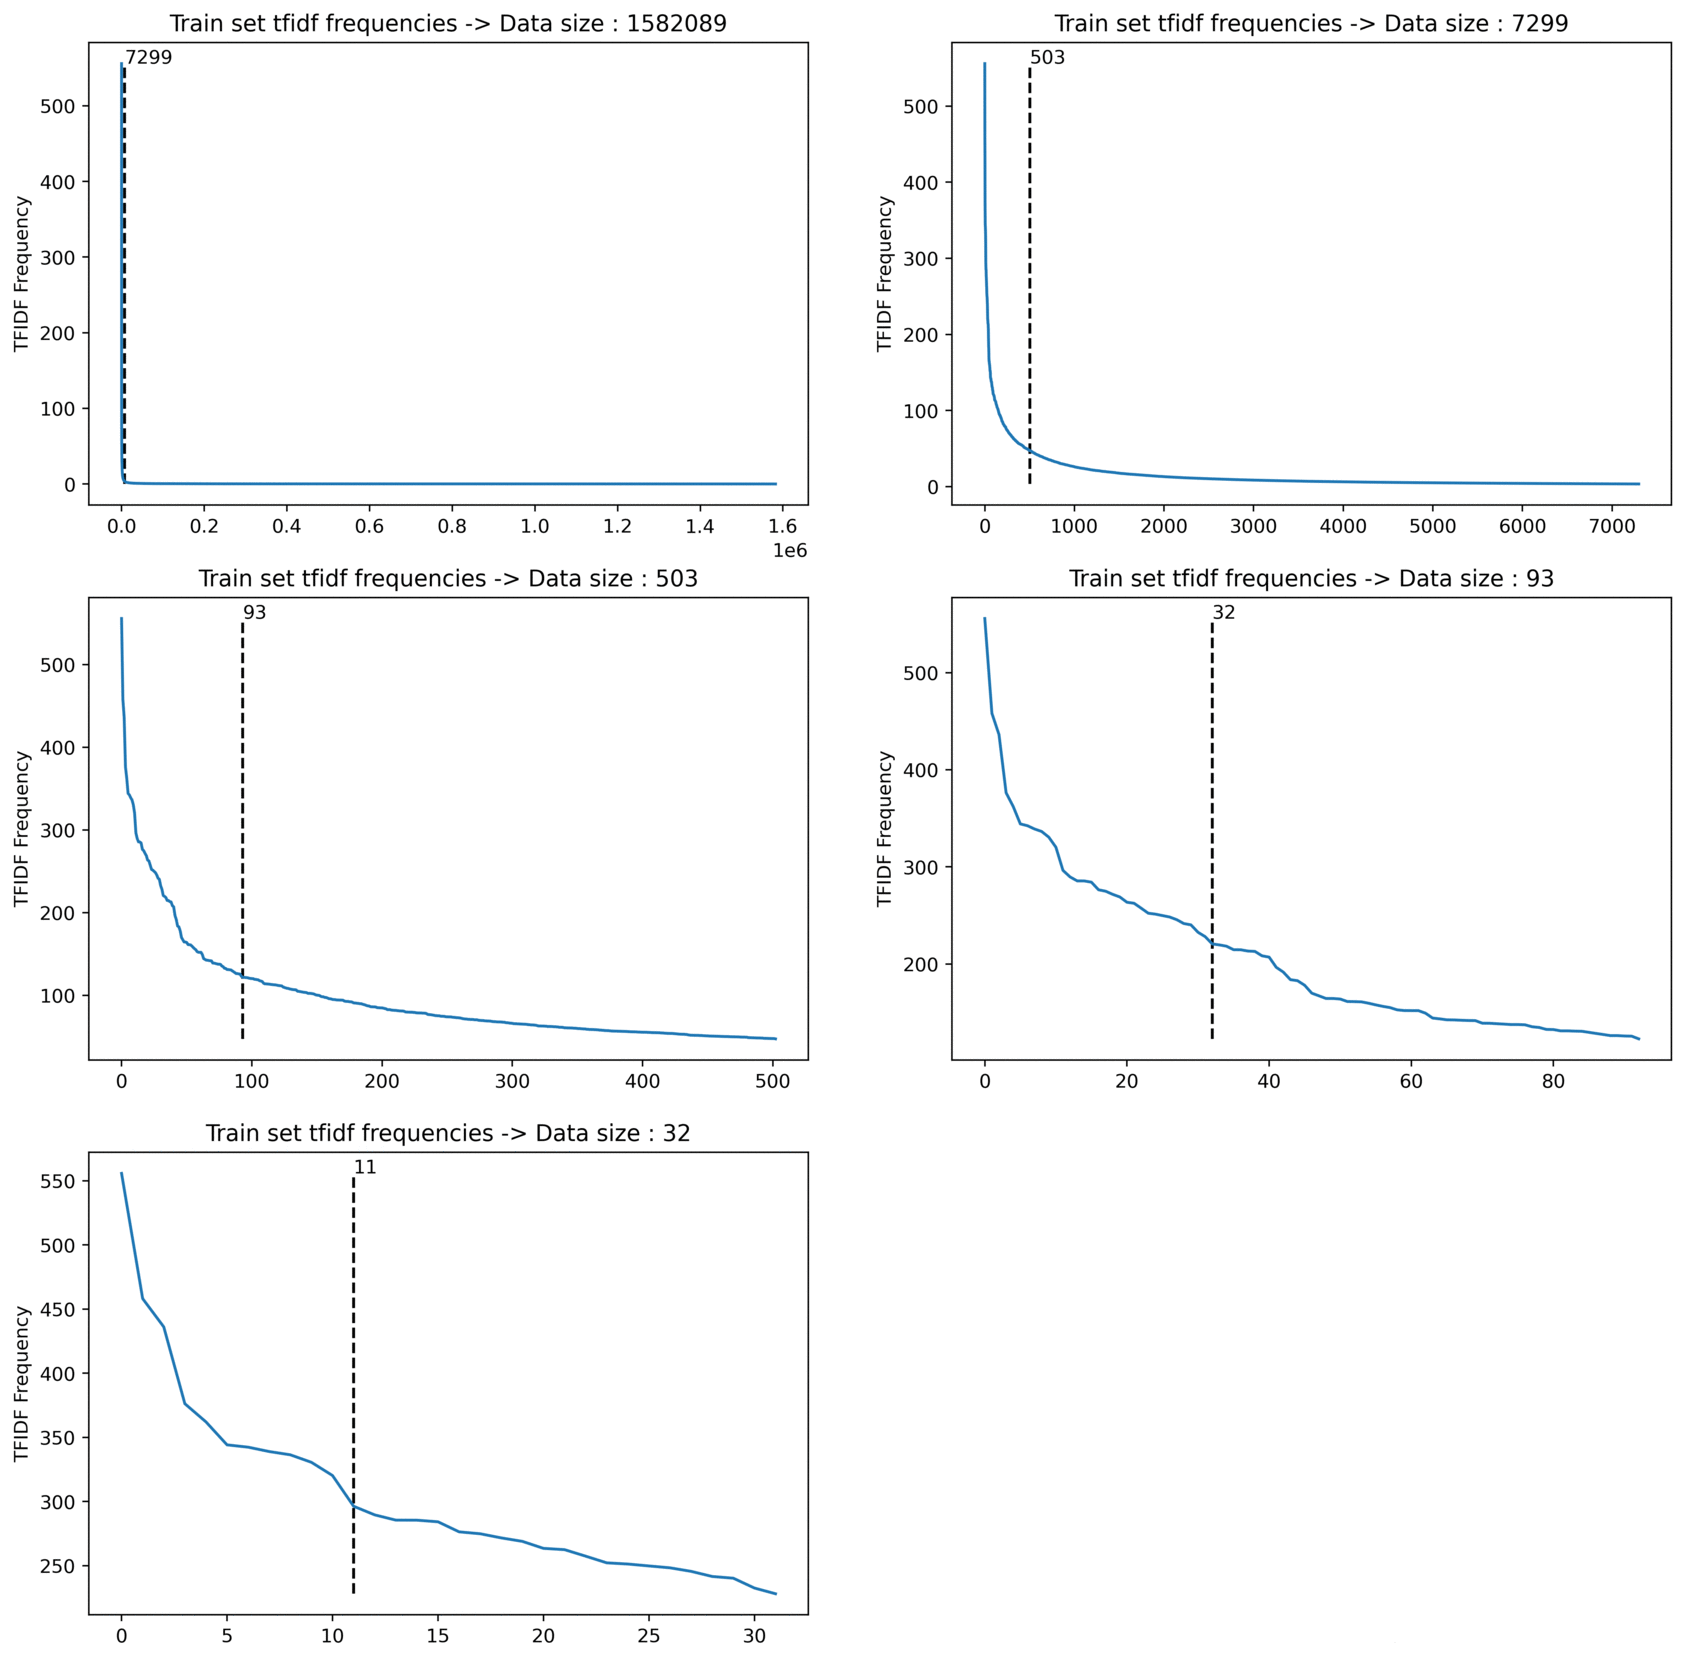
\includegraphics[width=0.5\textwidth,keepaspectratio]{figures/all_graphics.png}
\caption{Sequências de gráficos frequências TF*IDF com o \textit{knee\textunderscore{point}}}
\label{diagram:data_all_knee}
\centering
\end{center}
\end{figure}

\item \textbf{Conversão da lista de \textit{tokens} para uma matriz de \textit{TF features} usando o novo vocabulário reduzido na etapa anterior} 

Após o processo de segmentação do vocabulário, o numero de \textit{features} escolhido foi 600 termos.

Neste processo foi usado o algoritmo \textbf{\textit{TF}}, que mapeia a frequência de um termo tendo em conta o vocabulário definido anteriormente. Com estes valores temos uma noção de quantas vezes as palavras mais importantes são usadas nos documentos do \textit{dataset}.
\end{enumerate}

Após estas etapas os dados estão prontos para transitar para a fase de treino.
